\subsection{Les types de bases de données NoSql :}
Dans la mouvance NoSQL, il existe une diversité d’approches classées en quatre catégories. Ces différents systèmes NoSQL utilisent des technologies forts distinctes. Les différents modèles de structure sont décrits comme suit :

\subsubsection{Les bases de données orientées clé-valeur:}
Souvent assimilé à une « hashmap » distribuée, le système de base de données de type clé/valeur est probablement le plus connu et le plus basique que comporte la mouvance NoSQL. Son principe est extrêmement simple : chaque objet (valeur) est identifié par une clé unique. Celle-ci représente la seule manière de solliciter l’objet.

La communication avec la base de données se résume aux opérations basiques que sont PUT, GET, UPDATE et DELETE. La plupart des bases de données de type clé/valeur disposent d’une interface HTTP REST qui permet de procéder très facilement à des requêtes depuis n’importe quel langage de développement. Ces systèmes affichent des performances exceptionnellement élevées en lecture et en écriture, ainsi qu’une « scalabilité » horizontale étendue, cela vient du fait que ces types de bases sont réduits à un simple accès disque.

Du fait que les opérations possibles soient basiques (simple CRUD), le besoin en « scalabilité » verticale est fortement réduit. Ces systèmes sont souvent utilisés comme dépôts de données si toutefois les besoins en termes de requêtes restent de niveau simple et que l’intégrité relationnelle des données est non significative.

\begin{figure}[h]
	\centering
    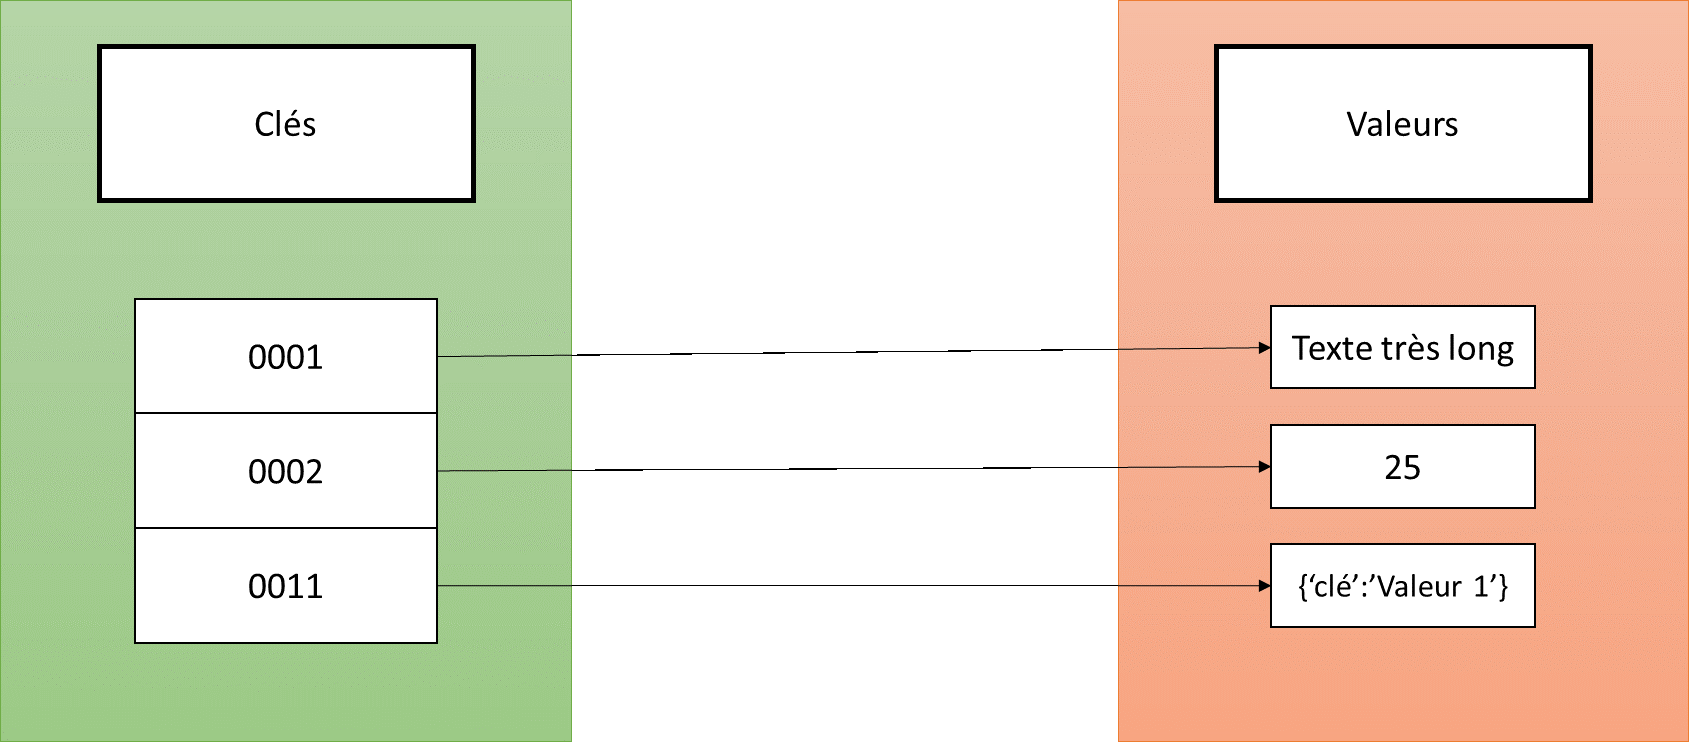
\includegraphics[scale=0.5]{img/part1/4.3}
    \caption{base de donnée orientée clé-valeur}
\end{figure}

\textit{\textbf{Exemple d'applications :} Détection de fraude en temps réel, IoT, e-commerce, gestion de cache, transactions rapides.}

\subsubsection{Les bases de données orientées colonnes}
La représentation orientée colonnes est celle qui se rapproche le plus des tables dans une base de données relationnelles. Elles permettent d'être beaucoup plus évolutive et flexible puisqu'on peut disposer de colonnes différentes pour chaque ligne. Elles peuvent évoluer dynamiquement en nombre et en nom et contrairement à une table relationnelle (pas de champ « NULL »).

\begin{figure}[h]
	\centering
    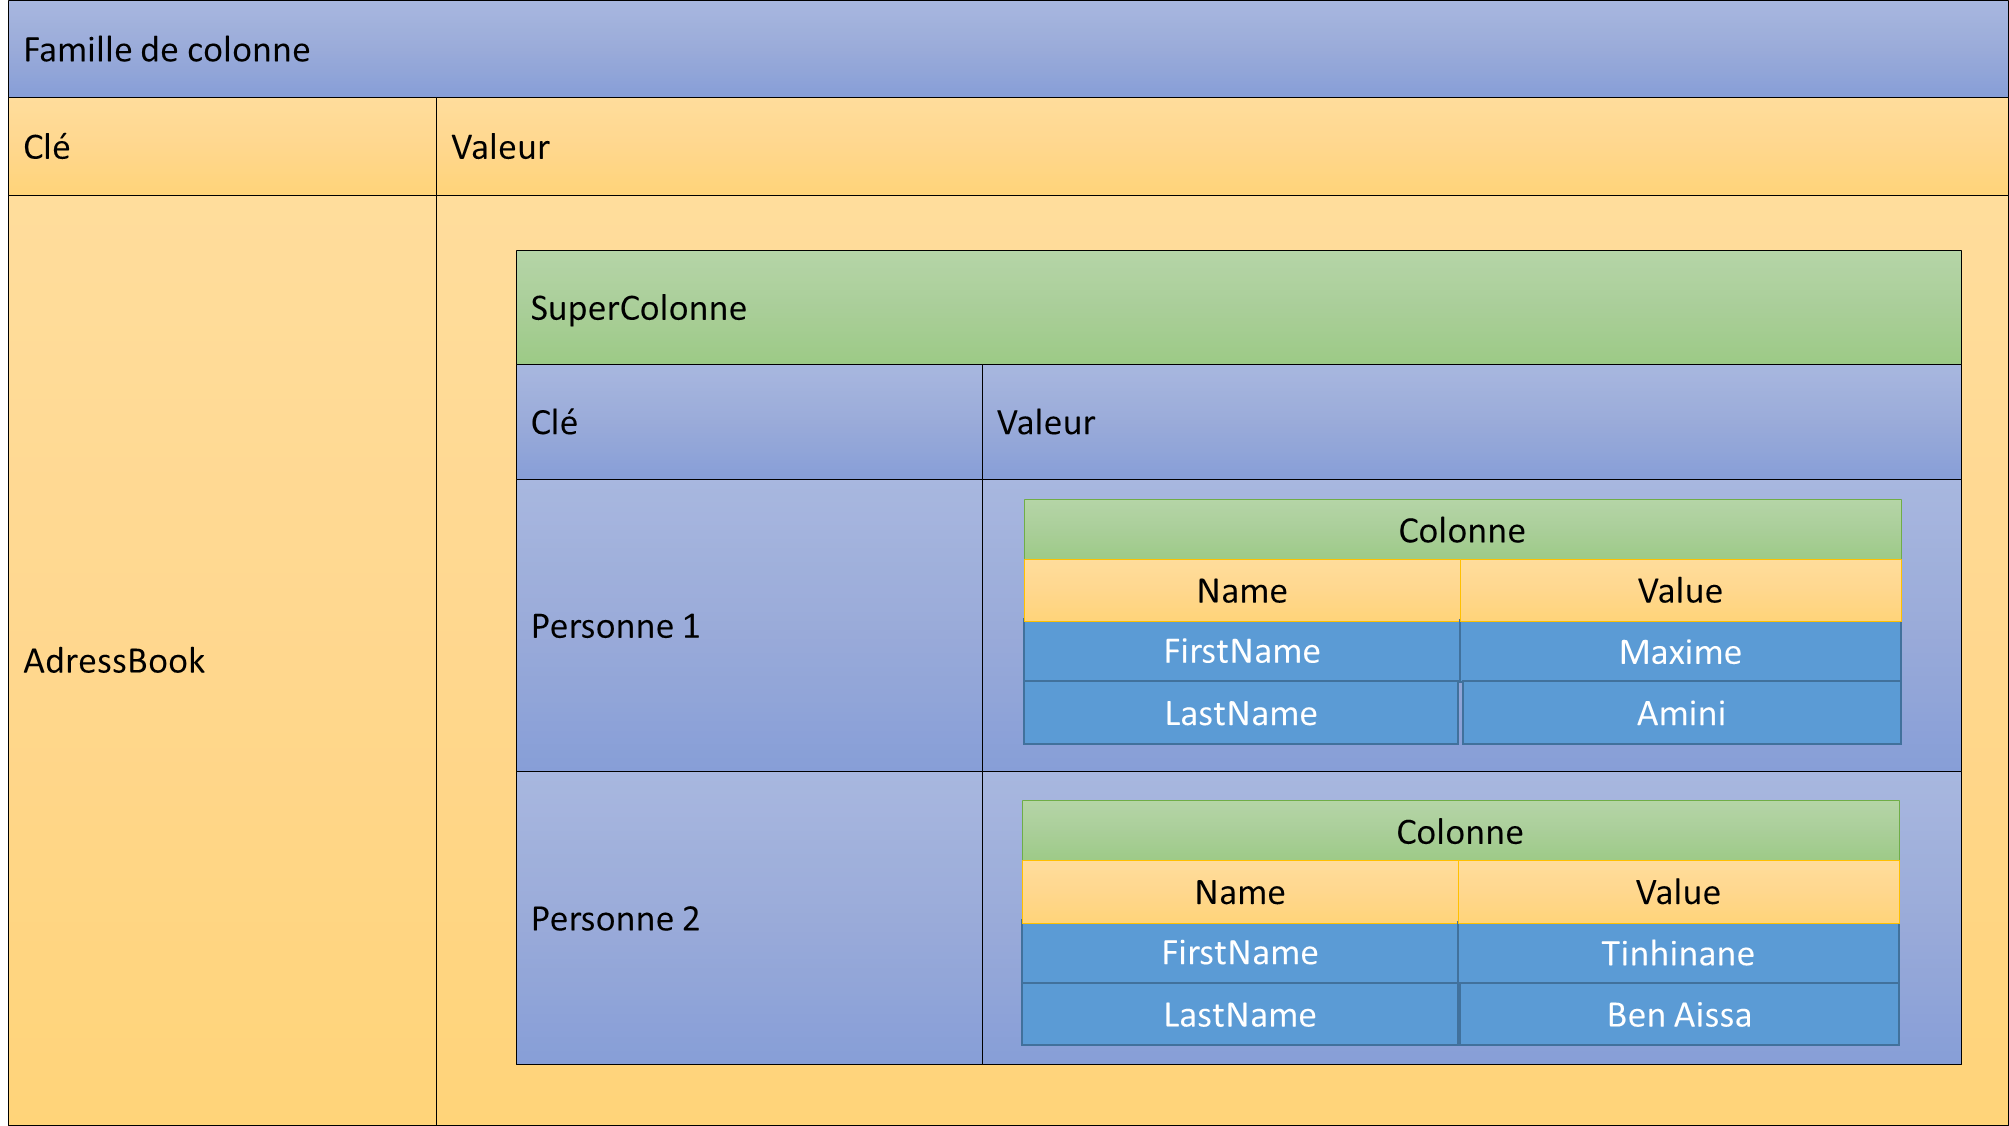
\includegraphics[scale=0.26]{img/part1/4.4}
    \caption{base de donnée orientée colonne}
\end{figure}
\bigskip \bigskip \bigskip  \bigskip  \bigskip 
\begin{itemize}[label=\textbullet]
\item \textbf{Column :} c’est l’entité de base qui représente un champ de données. Toutes les colonnes sont définies par un couple clé/valeur
\item \textbf{Super column :} c’est une colonne qui contient d’autres colonnes
\item \textbf{Column family :} elle est considérée comme un conteneur de plusieurs colonnes ou super-colonnes
\end{itemize}

\textit{\textbf{Exemple d'applications :} Comptage (vote en ligne, compteur, etc), journalisation, recherche de produits dans une catégorie, reportage à large échelle.}

\subsubsection{Les bases de données orientées documents}
Les systèmes de type documentaire sont composés de collections de documents. La représentation en document est une sorte d’extension du concept clé/valeur. La valeur est représentée sous forme de document, ces documents ont une structure arborescente : il contient une liste de champs, un champ est associé à une valeur qui peut, elle même être une liste. Ces documents sont principalement de type JSON ou XML.

Ces bases sont dites \textbf{« Schemaless »} ce qui signifie sans schéma défini. Cela veut tout simplement dire qu’il n’est pas nécessaire de définir au préalable les champs dans le document : on peut très bien en rajouter en cours de développement. Les documents peuvent être très différents les uns des autres au sein de la base. Le fait que les documents soient structurés permet d’effectuer des requêtes sur le contenu des objets.

\begin{figure}[h]
	\centering
    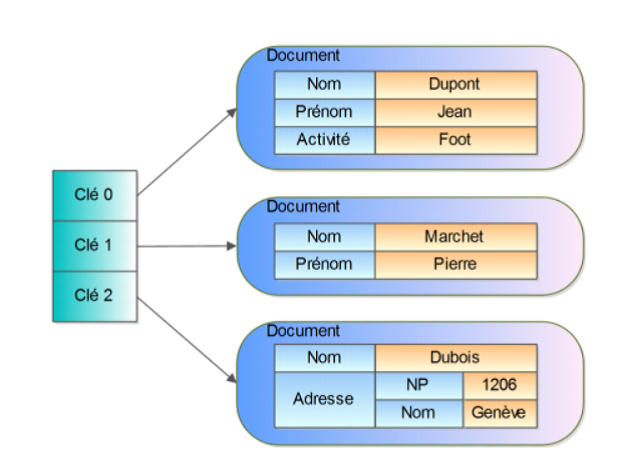
\includegraphics[scale=0.5]{img/part1/4.5}
    \caption{base de donnée orientée document}
\end{figure}

\textit{\textbf{Exemple d'applications :} Gestion de contenu (bibliothèques numériques, collections de produits, dépôts de logiciels, collections multimédia, etc.), framework stockant des objets, collection d'événements complexes, gestion des historiques d'utilisateurs sur réseaux sociaux.}

\subsubsection{Les bases de données orientées graphes}
Une base de données graphe établit des relations entre les données à l'aide de nœuds et d'arêtes. Le réseau de relation des données est organisé par les points nodaux et leurs connexions les uns avec les autres. Dans le cas de volumes de données aux informations fortement interconnectées, les bases de données graphiques NoSQL présentent une performance considérablement supérieure à celle des bases de données SQL relationnelles. 

Elles sont principalement utilisées dans le domaine des réseaux sociaux, pour représenter, par exemple, les relations entre les abonnés sur Twitter ou Instagram.

\begin{figure}[h]
	\centering
    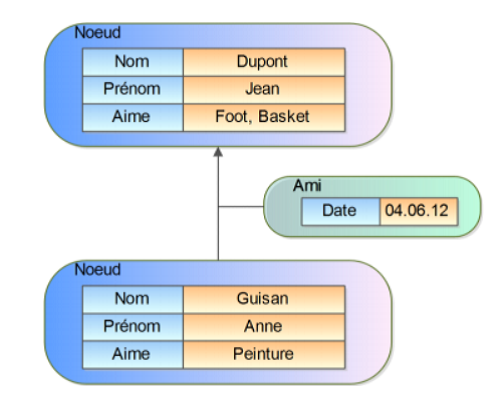
\includegraphics[scale=0.5]{img/part1/4.6}
    \caption{base de donnée orientée graphe}
\end{figure}

\textit{\textbf{Exemple d'applications :} Réseaux sociaux (recommandation, plus court chemin, cluster...), réseaux SIG 12 (routes, réseau électrique, fret...), web social (Linked Data).}

\subsubsection{Autres base de données}
Il existe plusieurs autres bases de données suivant une approche non relationnelle, mais elles ne sont pas considérées comme des bases de données NoSQL de base, mais plutôt comme des bases de données NoSQL logicielles :

\paragraph{Bases de données d'objets :} Les bases de données d'objets utilisent l'idée d'objets dans les langages de programmation et la transforment en systèmes de bases de données.

\textit{\textbf{Exemple :} db4o est un système de gestion de base de données orientée objet Open Source pour des applications Java et .Net 13.}

\paragraph{Bases de données XML :} Les bases de données XML sont vraiment des bases de données non SQL. Le langage de requête est XQuery, XPath ou XUpdate et non plus SQL. Ces bases de données permettent de stocker des données au format XML. Par conséquent, la structure de la base de données est hiérarchique. XML est largement utilisé dans les applications Internet, donc une transformation de (anciennement) SQL en XML n'est plus nécessaire.

\textit{\textbf{Exemple :} eXist est une base de données XML basée sur Java open source prenant en charge XQuery et XPath et possède comme CouchDB une interface HTTP RESTful.}


